% ****************************************************************************************** % Dissertation template and document class for Princeton University
% Author  : Jeffrey Scott Dwoskin <jdwoskin@princeton.edu>
% Adapted from: http://www.math.princeton.edu/graduate/tex/puthesis.html
% ****************************************************************************************** %


%%% For print copies
%% set 'singlespace' option to set entire thesis to single space, and define "\printmode" to remove all hyperlinks for printed copies of the thesis. Delete all output files before changing this mode -- it will turn hyperref package on and off
%\documentclass[12pt,lot, lof, singlespace]{puthesis}
%\newcommand{\printmode}{}

%%% For the electronic copy, use doublespacing, define "\proquestmode" to use outlined links, instead of colored links. 
\documentclass[12pt,lot, lof]{puthesis}
\newcommand{\proquestmode}{}
% I prefer proquestmode to be off for electronic copies for normal use, since the colored links are less distracting. However when printed in black and white, the colored links are difficult to read. 

%%% For early drafts without some of the frontmatter
% Also see the "ifodd" command below to disable more frontmatter
%\documentclass[12pt]{puthesis}

%%%%%%%%%%%%%%%%%%%%%%%%%%%%%%%%%%%%%%%%%%%%%%%%%%%%%%%%%%%%%\
%%%% Author & title page info

\title{Three Dimensional Palmprint Recognition}

\submitted{June 2012}  % degree conferral date (January, April, June, September, or November)
\copyrightyear{2012}  % year in which the copyright is secured by publication of the dissertation.
\author{Pei Qing}
\adviser{Professor David Zhang}  %replace with the full name of your adviser
%\departmentprefix{Program in}  % defaults to "Department of", but programs need to change this.
\department{Computing}

%%%%%%%%%%%%%%%%%%%%%%%%%%%%%%%%%%%%%%%%%%%%%%%%%%%%%%%%%%%%%\
%%%% Tweak float placements
% From: http://mintaka.sdsu.edu/GF/bibliog/latex/floats.html "Controlling LaTeX Floats"
% and based on: http://www.tex.ac.uk/cgi-bin/texfaq2html?label=floats
% LaTeX defaults listed at: http://people.cs.uu.nl/piet/floats/node1.html

% Alter some LaTeX defaults for better treatment of figures:
    % See p.105 of "TeX Unbound" for suggested values.
    % See pp. 199-200 of Lamport's "LaTeX" book for details.
    %   General parameters, for ALL pages:
    \renewcommand{\topfraction}{0.85}	% max fraction of floats at top
    \renewcommand{\bottomfraction}{0.6}	% max fraction of floats at bottom
    %   Parameters for TEXT pages (not float pages):
    \setcounter{topnumber}{2}
    \setcounter{bottomnumber}{2}
    \setcounter{totalnumber}{4}     % 2 may work better
    \setcounter{dbltopnumber}{2}    % for 2-column pages
    \renewcommand{\dbltopfraction}{0.66}	% fit big float above 2-col. text
    \renewcommand{\textfraction}{0.15}	% allow minimal text w. figs
    %   Parameters for FLOAT pages (not text pages):
    \renewcommand{\floatpagefraction}{0.66}	% require fuller float pages
	% N.B.: floatpagefraction MUST be less than topfraction !!
    \renewcommand{\dblfloatpagefraction}{0.66}	% require fuller float pages

% The documentclass already sets parameters to make a high penalty for widows and orphans. 

%%%%%%%%%%%%%%%%%%%%%%%%%%%%%%%%%%%%%%%%%%%%%%%%%%%%%%%%%%%%%\
%%%% Use packages

%\usepackage{amsfonts}

%%% For figures
\usepackage{graphicx}
%\usepackage{subfig,rotate}

%%% for comments
\usepackage{verbatim}

%%% For tables
\usepackage{multirow}
% Longtable lets you have tables that span multiple pages.
\usepackage{longtable}

% Booktabs produces far nicer tables than the standard LaTeX tables.
%   see: http://en.wikibooks.org/wiki/LaTeX/Tables
\usepackage{booktabs}

%set parameters for longtable:
% default caption width is 4in for longtable, but wider for normal tables
\setlength{\LTcapwidth}{\textwidth}



%%%%%%%%%%%%%%%%%%%%%%%%%%%%%%%%%%%%%%%%%%%%%%%%%%%%%%%%%%
%%% Printed vs. online formatting
\ifdefined\printmode

% Printed copy
% url package understands urls (with proper line-breaks) without hyperlinking them
\usepackage{url}


\else

\ifdefined\proquestmode
%ProQuest copy -- http://www.princeton.edu/~mudd/thesis/Submissionguide.pdf

% ProQuest requires a double spaced version (set previously). They will take an electronic copy, so we want links in the pdf, but also copies may be printed or made into microfilm in black and white, so we want outlined links instead of colored links.
\usepackage{hyperref}
\hypersetup{bookmarksnumbered}

% copy the already-set title and author to use in the pdf properties
\makeatletter
\hypersetup{pdftitle=\@title,pdfauthor=\@author}
\makeatother

\else
% Online copy

% adds internal linked references, pdf bookmarks, etc

% turn all references and citations into hyperlinks:
%  -- not for printed copies
% -- automatically includes url package
% options:
%   colorlinks makes links by coloring the text instead of putting a rectangle around the text.
\usepackage{hyperref}
\hypersetup{colorlinks,bookmarksnumbered}

% copy the already-set title and author to use in the pdf properties
\makeatletter
\hypersetup{pdftitle=\@title,pdfauthor=\@author}
\makeatother

% make the page number rather than the text be the link for ToC entries
%\hypersetup{linktocpage}
\fi % proquest or online formatting
\fi % printed or online formatting


%%%%%%%%%%%%%%%%%%%%%%%%%%%%%%%%%%%%%%%%%%%%%%%%%%%%%%%%%%%%%\
%%%% Define commands

% Define any custom commands that you want to use.
% For example, highlight notes for future edits to the thesis
%\newcommand{\todo}[1]{\textbf{\emph{TODO:}#1}}


% create an environment that will indent text
% see: http://latex.computersci.org/Reference/ListEnvironments
% 	\raggedright makes them left aligned instead of justified
\newenvironment{indenttext}{
    \begin{list}{}{ \itemsep 0in \itemindent 0in
    \labelsep 0in \labelwidth 0in
    \listparindent 0in
    \topsep 0in \partopsep 0in \parskip 0in \parsep 0in
    \leftmargin 1em \rightmargin 0in
    \raggedright
    }
    \item
  }
  {\end{list}}

% another environment that's an indented list, with no spaces between items -- if we want multiple items/lines. Useful in tables. Use \item inside the environment.
% 	\raggedright makes them left aligned instead of justified
\newenvironment{indentlist}{
    \begin{list}{}{ \itemsep 0in \itemindent 0in
    \labelsep 0in \labelwidth 0in
    \listparindent 0in
    \topsep 0in \partopsep 0in \parskip 0in \parsep 0in
    \leftmargin 1em \rightmargin 0in
    \raggedright
    }

  }
  {\end{list}}



%%%%%%%%%%%%%%%%%%%%%%%%%%%%%%%%%%%%%%%%%%%%%%%%%%%%%%%%%%%%%\
%%%% Front-matter

% For early drafts, you may want to disable some of the frontmatter. Simply change this to "\ifodd 1" to do so.
\ifodd 0
% front-matter disabled while writing chapters
\renewcommand{\maketitlepage}{}
\renewcommand*{\makecopyrightpage}{}
\renewcommand*{\makeabstract}{}

% you can just skip the \acknowledgements and \dedication commands to leave out these sections.

\else


\abstract{
% Abstract can be any length, but should be max 350 words for a Dissertation for ProQuest's print indicies (150 words for a Master's Thesis) or it will be truncated for those uses.
%!TEX root = thesis.tex

Three Dimensional (3D) palmprint has proved to be a significant biometrics for personal authentication. 3D palmprints are harder to counterfeit than 2D palmprints and more robust to variations in illumination and serious scrabbling on the palm surface. Previous work on 3D palmprint recognition has concentrated on local features such as texture and lines.

% a blank line as required
\vspace{12pt}

In this dissertation, the authentication process are improved using 3D features. The features are stable in samples from a single person over time and distinguishable among samples from different people. Three features adopted are Maximum Depth of palm center, Horizontal Cross-section Area and Radial Line Length from the centroid to the boundary of 3D palmprint horizontal cross-section of different levels. The feature set is combined as a column feature vector for matching. Support Vector Machine is introduced for higher efficiency.

% a blank line as required
\vspace{12pt}

Experiments are conducted on an existing 3D palmprint database of 8,000 samples. The results show that the proposed method is able to achieve an reasonable performance.


% \textbf{Keywords}: 3D palmprint identification, 3D palmprint verification, SVM

}

\acknowledgements{
%I would like to thank...
I would like to thank the Math department for providing the original documentclass file that this class is based upon. I would like to thank my parents, without whom my life would not be possible. I would also like to thank my advisor, my dissertation committee, and my research collaborators because every graduate student needs to do so. And finally, I thank the members of my research group, to whom I leave this template to save you some of the trouble I had to go through getting my dissertation to compile in \LaTeX{}.  

Don't forget to ask your advisor if your work was sponsored by a grant that needs to be acknowledged in this section.  
}

\dedication{To my parents.}

\fi  % disable frontmatter


%%%%%%%%%%%%%%%%%%%%%%%%%%%%%%%%%%%%%%%%%%%%%%%%%%%%%%%%%%%%%\
%%%% Hide some chapters

%%% If you want to produce a pdf that includes only certain chapters, specify them with includeonly, in addition to including all chapters below.
%\includeonly{ch-intro/chapter-intro}
%%% You can also specify multiple chapters.
%\includeonly{ch-intro/chapter-intro,ch-usage/chapter-usage}
%\includeonly{chap1,chap2,chap3}


%%%%%%%%%%%%%%%%%%%%%%%%%%%%%%%%%%%%%%%%%%%%%%%%%%%%%%%%%%%%%
%%%% Notes:

% Footnotes should be placed after punctuation.\footnote{place here.}
% Generally, place citations before the period~\cite{anotherauthor}.
% The proper usage for i.e., and e.g., include commas ``(e.g., option A, option B)''

%%%%%%%%%%%%%%%%%%%%%%%%%%%%%%%%%%%%%%%%%%%%%%%%%%%%%%%%%%%%%
%%%% Import chapters

\begin{document}

\makefrontmatter


% If you've disabled frontmatter, you can insert the toc manually
%\tableofcontents\clearpage

% \include lets us split up the document (and each include starts a new page):
%!TEX root = ../thesis.tex
\chapter{Introduction\label{ch:intro}}

Palmprint has been increasingly recognized as unique and stable biometric characteristics for personal authentication. In the past decade, various methods based on two dimensional (2D) palmprint have been studied in depth. The 2D recognition techniques have proved to achieve high accuracy~\cite{Kong:2009hj}.

In recent years, three dimensional (3D) palmprint recognition devices emerge and are quite promising because of the additional depth information gathered.

Although the devices has been out for more than two years, most previous matching algorithms treat 3D information as a supplement to 2D texture images and used joint matching techniques to increase accuracy~\cite{Li:2011ur, Li:2010en, Zhang:2009dp, Zhang:2008kc, Zhang:2010uu}. Authentication with only the 3D information has not been thoroughly studied. The amount of useful information carried by the 3D data is still under investigation.

There are two major challenges:

\begin{enumerate}
\item 3D devices, compared to 2D ones, are lower in resolution.
\item The depth values are susceptible to movements of human hands and are therefore less stable than 2D texture information of palmprints.
\end{enumerate}

David et al. explore a 3D palmprint recognition approach by exploiting the 3D structural information of the palm surface~\cite{Zhang:2009dp, Zhang:2008kc}. The structured light imaging is used to acquire the 3D palmprint data, from which several types of unique features, including mean curvature image, Gaussian curvature image, and surface type, are extracted. A fast feature matching and score-level fusion strategy is proposed for palmprint matching and classification. Wei et al. propose an efficient joint 2D and 3D palmprint matching scheme~\cite{Li:2010en}. The principal line features and palm shape features are extracted and used to accurately align the palmprint, and a couple of matching rules are defined to efficiently use the 2D and 3D features for recognition. Experiments show that the 3D features are not correlated with existing 2D ones and palmprint verification performance can be greatly improved by using both. Wei et al. also present an efficient scheme for 3D palmprint recognition~\cite{Li:2011ur}. They extract both line and orientation features by calculating and enhancing Gaussian-curvature and mean-curvature image or the 3D palmprint sample. The two types of features are then fused at either score level or feature level for the final 3D palmprint recognition.

Existing work has been done to utilize the 3D information for palmprint classification and sorting. The global features proposed for that purpose are fast in matching speed but low in accuracy compared to 2D techniques.

Three features are extracted from 3D palmprint depth data: Maximum Depth, Horizontal Cross-section Area and Radial Line Length. Theses features are combined together as a brief description of a 3D palmprint sample. Viewing the feature set as a column vector, various data processing techniques can be applied to improve the recognition efficiency such as dimension reduction and machine learning.

The rest of this work is organized as follows. Chapter \ref{ch:pastwork} briefly introduces the existing research efforts related to this topic. Chapter \ref{ch:methodology} describes the entire data processing procedures to extract features and use them for 3D palmprint recognition. Chapter \ref{ch:experiment} shows some experiment results. Chapter \ref{ch:conclusion} concludes the work and points out potentials for some future work.

%!TEX root = ../thesis.tex
\chapter{Related Work\label{ch:pastwork}}

This work is based on a number of previous research efforts. The samples are collected with an existing hardware device. And there also exist some efforts on recognition based on local features.

% include other files for sections of this chapter. These use the 'input' command since each section within a chapter should not start a new page.
% If you want to swap the order of sections, it is as simple as reversing the order you include them.
\section{Hardware}
\label{sec:pastwork:hardware}

% ~\cite{Li:2011ur,Li:2010en,Zhang:2009dp}

Different approaches are available for 3D imaging including laser scanning~\cite{Blais:1988te}, viewpoint reconstruction~\cite{Hartley:2000un} and structured light scanning~\cite{Halioua:1984ue}. Structured light scanning, compared to other approaches, is fast and accurate. For palmprint recognition, speed is an important factor. The verification or identification result must be given in a short time. Otherwise the system is barely suitable for real-world applications.

% http://en.wikipedia.org/wiki/Structured-light_3D_scanner

Projecting a narrow band of light onto a three-dimensionally shaped surface produces a line of illumination that appears distorted from other perspectives than that of the projector, and can be used for an exact geometric reconstruction of the surface shape (light section).

A faster and more versatile method is the projection of patterns consisting of many stripes at once, or of arbitrary fringes, as this allows for the acquisition of a multitude of samples simultaneously. Seen from different viewpoints, the pattern appears geometrically distorted due to the surface shape of the object.

\begin{figure}[htb]
  \begin{center}
    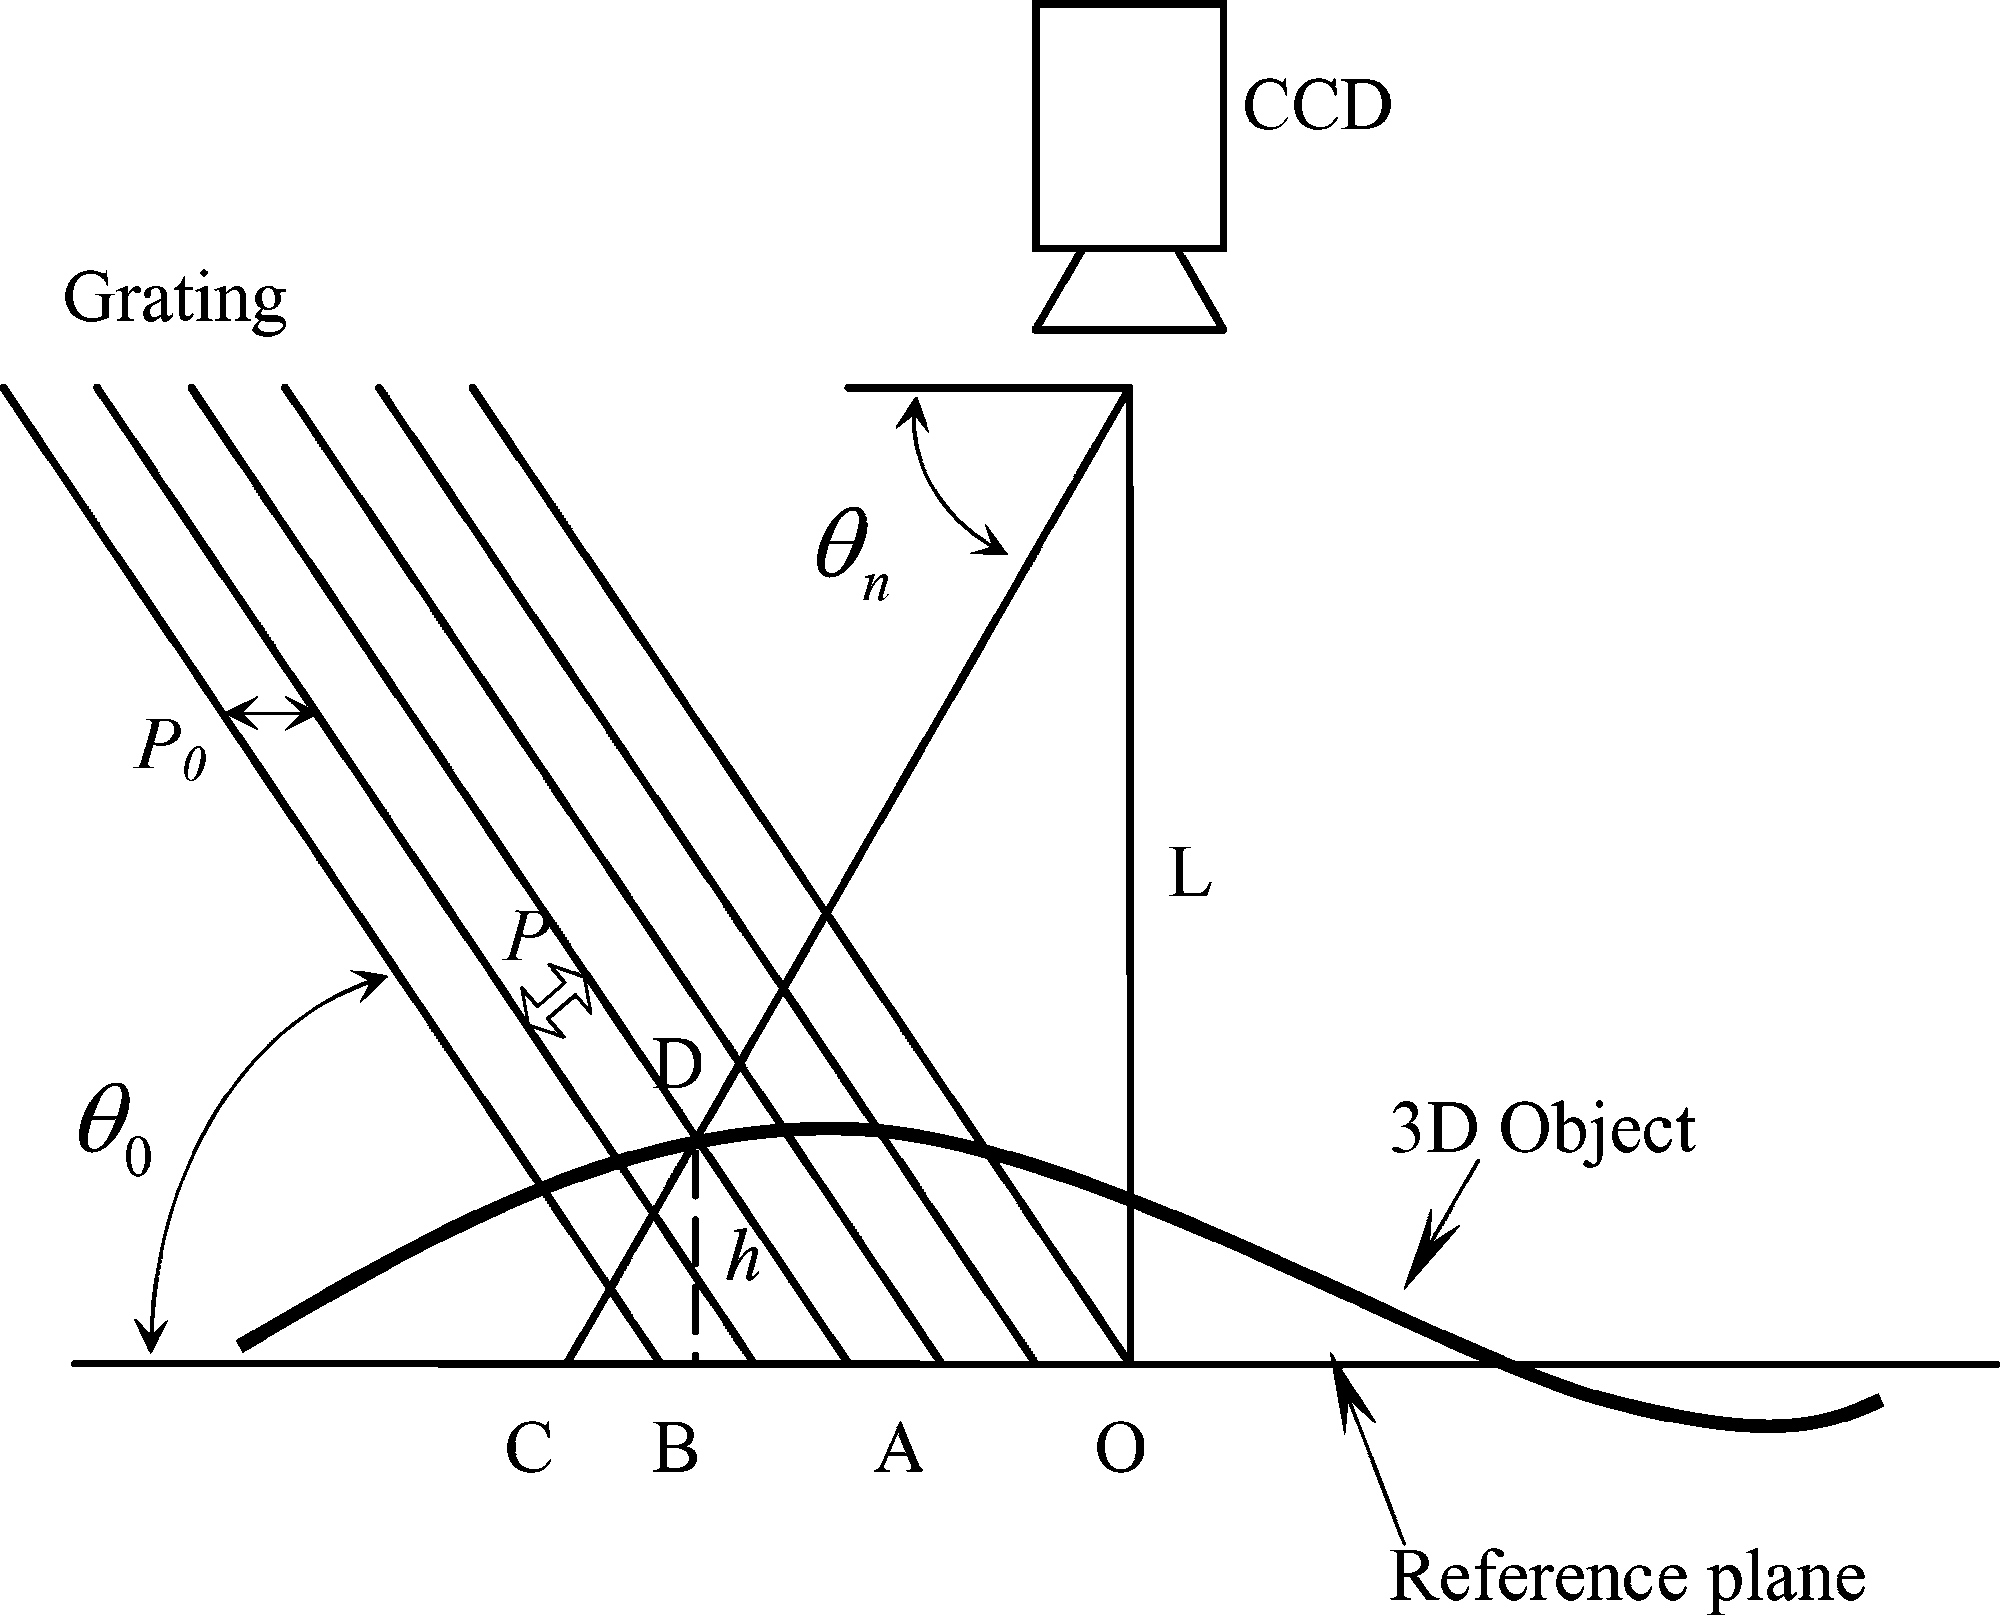
\includegraphics[width=0.9\linewidth]{ch-pastwork/figures/sli}
    \caption[The principle of structured-light imaging]{The principle of structured-light imaging\cite{Li:2009eq}}
    \label{fig:pastwork:sli}
  \end{center}
\end{figure}

Although many other variants of structured light projection are possible, patterns of parallel stripes are widely used. Figure~\ref{fig:pastwork:strippattern} shows the geometrical deformation of a strip pattern projected onto a palm. The displacement of the stripes allows for an exact retrieval of the 3D coordinates of any details on the palm's surface.

David et. al designed a 3D palmprint capturing device~\cite{Zhang:2008kc}. The system proposed has a resolution of 768x576.

\begin{figure}[htb]
  \begin{center}
    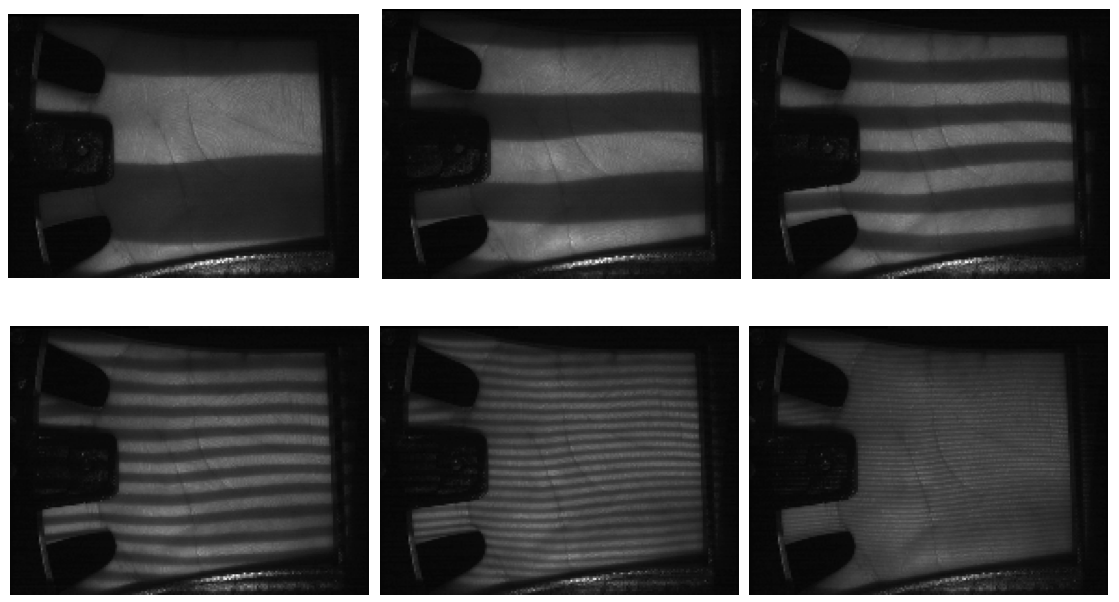
\includegraphics[width=0.9\linewidth]{ch-pastwork/figures/strippattern}
    \caption[Sample patterns of the stripes on the palm]{Sample patterns of the stripes on the palm~\cite{Li:2009eq}}
    \label{fig:pastwork:strippattern}
  \end{center}
\end{figure}

\section{Recognition Methods}
\label{sec:pastwork:recogmethods}

Traditionally, palmprint recognition has made use of either high or low resolution 2D palmprint images. High resolution images are suitable for forensic applications [3] while low resolution images are suitable for civil and commercial applications [4]. Most current research use low resolution palmprint recognition and is either texture-based or line-based. The texture-based methods include PalmCode [4], Competitive Code [5] and Ordinal Code [6]. These methods use a group of filters to enhance and extract the phase or directional features which can represent the texture of the palmprint. Line-based methods use line or edge detectors to explicitly extract line information from the palmprint that is then used for matching. The representative methods include Derivative of Gaussian based line extraction [7] and Modified Finite Radon transform (MFRAT) based line extraction [8].

In recent years, 3D techniques have been applied to biometric authentication, such as 3D face [9] and 3D ear recognition [10]. Most recently, a structured-light imaging [11, 12] 3D palmprint system [13] was developed that captures the depth information of a palmprint. This information is then used to calculate the Mean and the Gaussian curvatures for use in 3D palmprint matching and recognition. To date, however, there has been no work with 3D palmprints that has extracted global shape features, which may be useful in classification and indexing. For fingerprint, according to the global ridge structure and singularities, it can be classified into five classes: arch, tented arch, left loop, right loop and whorl [14]. Wu et al. classified the palmprint into six classes according to the palmprint principal lines [15]. Besides the exclusive classification technique, the continuous classification technique is also widely used for indexing the database for personal identification [16].

Some general features were extracted for recognition including 3D Mean Curvature Image, 3D Gauss Curvature Image and 3D Surface Type~\cite{Zhang:2008kc,Li:2009eq}.





\chapter{Usage\label{ch:usage}}

To start, in your main .tex file, use this class as your main documentclass instead of `report' or `book'. For example:
\begin{quote}
$\backslash documentclass[12pt,lot, lof]\{puthesis\}$
\end{quote}

In this example, we setup our document to use the PU Thesis style, with 12pt font for body text, and to include a List of Tables and List of Figures in the front matter. You could instead set an 11 point or 10 point font by changing the first option. You can also add `los' to include a list of symbols.

To use single spacing, add the option `singlespace'. This is a special option for the \texttt{puthesis} documentclass, which sets single spacing for both the front matter and for the document itself. Additional parameters should be set in your main .tex file, and are described in detail in Section~\ref{sec:usage:options}.

The template itself declares two other options, to be set immediately after the \texttt{documentclass} command. First is `printmode', declared with the command:
\begin{quote}
$\backslash newcommand\{\backslash printmode\}\{\}$
\end{quote}
This command, used later in the thesis.tex file, turns off the \texttt{hyperref} package and all internal links in the PDF file. This removes any colored links and highlighting that would not be appropriate in a printed and bound thesis. Instead the \texttt{url} package is loaded, so that \\url commands in your document will continue to work and urls will break properly across multiple lines.

When `printmode' is not specified, the hyperref package is included. It creates colored links for citations, footnotes, and internal references, which can be used to navigate the PDF document more easily. It also adds bookmarks to the PDF file, mirroring the table of contents. By default, it is set to use colored links. For the PDF file that you will submit electronically to ProQuest, this may not be desirable since some copies may be printed, while others will be used electronically. Thus another option, `proquestmode', is defined that keeps hyperref but disables colored links:
\begin{quote}
$\backslash newcommand\{\backslash proquestmode\}\{\}$
\end{quote}
This mode has no effect when used in combination with `printmode'. 


\section{Options}
\label{sec:usage:options}

In this section, we describe the options you can set when using this thesis class.
\tablespacing
% tablespacing is defined by the class to set single spacing for the long table when in doublespacing mode. If the singlespace option is set, this command has no effect.

\begin{longtable}{p{0.3\linewidth} p{0.6\linewidth}}

  % First page heading
  \caption[Options Provided by the PUthesis Class]{List of options for the puthesis document class and template} \label{tab:usage:options}\\
  \toprule
  \textbf{Option} & \textbf{Description} \\
  \midrule
  \endfirsthead

  % Future page heading
  \caption[]{(continued)}\\
  \toprule
  \textbf{Option} & \textbf{Description} \\
  \midrule
  \endhead

  % Page footer
  \midrule
  \multicolumn{2}{r}{(Continued on next page)}\\
  \endfoot

  % Last page footer
  \bottomrule
  \endlastfoot

  12pt &
  Specify the font size for body text as a parameter to \texttt{documentclass}. The Mudd Library requirements~\cite{muddthesis2009} state that 12pt is preferred for serif fonts (e.g., Times New Roman) and 10pt for sans-serif fonts (e.g., Arial).
  \\

  letterpaper &
  If your document is coming out in a4paper, your LaTeX defaults may be wrong. Set this option as a parameter to \texttt{documentclass} to have the correct 8.5"x11" paper size.
  \\

  lot &
  Set this option as a parameter to \texttt{documentclass} to insert a List of Tables after the Table of Contents.
  \\


  lof &
  Set this option as a parameter to \texttt{documentclass} to insert a List of Figures after the Table of Contents and the List of Figures.
  \\

  los &
  Set this option as a parameter to \texttt{documentclass} to insert a List of Symbols after the Table of Contents and the other lists.
  \\

  singlespace &
  Set this option as a parameter to \texttt{documentclass} to single space your document. Double spacing is the default otherwise, and is required for the electronic copy you submit to ProQuest. Single spacing is permitted for the printed and bound copies for Mudd Library.
  \\
  
  draft &
  Set this option as a parameter to \texttt{documentclass} to have \LaTeX mark sections of your document that have formatting errors (e.g., overfull hboxes). 
  \\

  % the cmidrule here spans both columns but is indented slightly on the left and right. 
  \cmidrule[0.1pt](l{0.5em}r{0.5em}){1-2}

  \raggedright
  $\backslash newcommand$ $\{\backslash printmode\}\{\}$ &
  Insert this command after the \texttt{documentclass} command to turn off the hyperref package to produce a PDF suitable for printing.
  \\

  \raggedright
  $\backslash newcommand$ $\{\backslash proquestmode\}\{\}$  &
  Insert this command after the \texttt{documentclass} command to turn off the `colorlinks' option to the hyperref package. Links in the pdf document will then be outlined in color instead of having the text itself be colored. This is more suitable when the PDF may be viewed online or printed by the reader.
  \\

  $\backslash makefrontmatter$ &
  Insert this command after the \texttt{$\backslash begin\{document\}$} command, but before including your chapters to insert the Table of Contents and other front matter.
  \\
  
  \cmidrule[0.1pt](l{0.5em}r{0.5em}){1-2}

  $\backslash title$ &
  Set the title of your dissertation. Used on the title page and in the PDF properties.
  \\

  $\backslash submitted$ &
  Set the submission date of your dissertation. Used on the title page. This should be the month and year when your degree will be conferred, generally only January, April, June, September, or November. Check the Mudd Library rules~\cite{mudd2009} for the appropriate deadlines.
  \\

  $\backslash copyrightyear$ &
  Set the submission year of your dissertation. Used on the copyright page.
  \\

  $\backslash author$ &
  Your full name. Used on the title page, copyright page, and the PDF properties. \\

  $\backslash adviser$ &
  Your adviser's full name. Used on the title page. \\

  $\backslash departmentprefix$ &
  The wording that precedes your department or program name. Used on the title page. The default is ``Department of'', since most people list their department and can leave this out (e.g., Department of Electrical Engineering), however if yours is a program, set $\backslash departmentprefix\{Program in\}$ \\

  $\backslash department$ &
  The name of your department or program. Used on the title page. \\

  \cmidrule[0.1pt](l{0.5em}r{0.5em}){1-2}
  
  \raggedright  
  $\backslash renewcommand$ $\{\backslash maketitlepage\}\{\}$ &
  Disable the insertion of the title page in the front matter. This is useful for early drafts of your dissertation. \\

  \raggedright  % full justification places the * in an awkward place
  $\backslash renewcommand*\{\backslash makecopyrightpage\}\{\}$ &
  Disable the insertion of the copyright page in the front matter. This is useful for early drafts of your dissertation. \\

  \raggedright 
  $\backslash renewcommand*\{\backslash makeabstract\}\{\}$ &
  Disable the insertion of the abstract in the front matter. This is useful for early drafts of your dissertation. \\

\end{longtable}
\bodyspacing
% bodyspacing restores double spacing or single spacing after the table

% need blank space after \bodyspacing

I've seen other people print their dissertations using $\backslash pagestyle\{headings\}$, which places running headings on the top of each page with the chapter number, chapter name, and page number. This documentclass is not currently compatible with this option -- the margins are setup to be correct with page numbers in the footer, placing them 3/4" from the edge of the paper, as required. If you wish to use headings, you will need to adjust the margins accordingly.
 





\chapter{Conclusions\label{ch:conclusion}}

\section{Summary}
% In this work, we explain how to use the puthesis.cls class file and the accompanying template.

In this dissertation, the authentication process are improved using 3D features. The features are stable in samples from a single person over time and distinguishable among samples from different people.

Three features adopted are Maximum Depth of palm center, Horizontal Cross-section Area and Radial Line Length from the centroid to the boundary of 3D palmprint horizontal cross-section of different levels. These cannot be extracted from 2D palmprints and are not correlated with local features, such as line and texture features. To make these global features efficient for use in coarse classification, we treat them as a multi-dimensional vector and use OLDA to map it to a lower dimensional space.

We then improve the efficiency of 3D palmprint recognition using two proposed approaches, coarse-level matching and RSVM, both of which significantly reduce the penetration rate during retrieval.

Experiments are conducted on an existing 3D palmprint database of 8,000 samples. The results show that the proposed method is able to achieve an reasonable performance.
 % Conclusion
%!TEX root = chapter-conclusion.tex
\section{Future Work}

As shown in Chapter ~\ref{ch:experiment}, the error rate in recognition using only the (Maximum Depth, Horizontal Cross-section Area, Radial Line Length are much higher than the cases when Mean Curvature Image is used. The problem with the latter one is its computation time.

The most interesting direction for future work is to find more descriptive and efficient features for the 3D ROI. % Future work

\appendix % all chapters following will be labeled as appendices
\chapter{Implementation Details\label{ch:implementation}}

Appendices are just chapters, included after the $\backslash appendix$ command.

\section{Switching Formats}
When switching \texttt{printmode} on and off (see Section~\ref{sec:usage:options}), you may need to delete the output .aux files to get the document code to compile correctly. This is because the hyperref package is switched off for \texttt{printmode}, but this package inserts extra tags into the contents lines in the auxiliary files for PDF links, and these can cause errors when the package is not used.

\section{Long Tables}

Long tables span multiple pages. By default they are treated like body text, but we want them to be single spaced all the time. The class therefore defines a new command, $\backslash tablespacing$, that is placed before a long table to switch to single spacing when the rest of the document is in double spacing mode. Another command, $\backslash bodyspacing$, is placed after the long table to switch back to double spacing. Normal tables using \texttt{tabular} automatically use single spacing and do not require the extra commands.

When the documentclass is defined with the `singlespace' option, these commands are automatically adjusted to stay in single spacing after the long table.

Make sure there is always at least one blank line after the $\backslash bodyspacing$ command before the end of the file.

Some times long tables do not format correctly on the first pass. If the column widths are wrong, try running the \LaTeX compiler one or two extra times to allow it to better calculate the column widths.

If you want your long table to break pages at a specific point, you can insert the command $\backslash pagebreak[4]$, to tell \LaTeX that it really should put a page break there. $\backslash pagebreak[2]$ gives it a hint that this is a good place for a page break, if needed. If there's a row that really should not be broken across a page, use $\backslash \backslash *$, which will usually prevent a pagebreak. 

\section{Booktabs}
The booktabs package is included to print nicer tables. See the package documentation~\cite{fear2005booktabs} for more details and motivation. Generally, all vertical lines are removed from the tables for a better visual appearance (so don't put them in), and better spacing and line thicknesses are used for the horizontal rules. The rules are defined as $\backslash toprule$ at the top of the table, $\backslash midrule$ in between the heading and the body of the table (or between sections of the table), and $\backslash bottomrule$ at the end of the table. $\backslash cmidrule$ can be used with the appropriate options to have a rule that spans only certain columns of the table.

\section{Bibliography and Footnotes}

The bibliography and any footnotes can also be single spaced, even for the electronic copy. The template is already setup to do this.

Bibliography entries go in the .bib file. As usual, be sure to compile the \LaTeX code, then run BibTeX, and then run \LaTeX again.

To cite websites and other electronically accessed materials, you can use the `@electronic' type of BibTeX entry, and use the `howpublished' field to include the URL of the source material.

The formatting of bibliography entries will be done automatically. Usually the titles are changed to have only the first word capitalized. If you'd prefer to have your original formatting preserved, place the title in an extra set of curly braces, i.e., ``title = \{\{My title has an AcroNyM that should stay unchanged\}\},''.

\section{Figures and Tables}
The captions of figures and tables take an optional parameter in square brackets, specifying the caption text to be used in the Table of Contents. The regular caption in curly braces is used for the table itself.

Generally captions for tables are placed above the table, while captions for figures are placed below the figure.




%!TEX root = ../thesis.tex
\chapter{Printing and Binding\label{ch:printing}}

\section{Printing}

For the library copies of your dissertation, you must use archival quality printing and binding. This means acid-free paper, containing at least 25\% cotton fiber. Triangle Repocenter on Nassau Street in Princeton offers both 25\% cotton paper and 100\% cotton paper. Most people choose the 25\% cotton paper, and this is generally recommended by the binders. The 100\% copy paper is somewhat thicker and the extra expense is unnecessary. 

Triangle offers online submission of your printing and binding order at: \url{http://triangleprinceton.com/collegiatebinding/thesis/}. If you request binding from them, they will deliver the paper copies to Smith-Shattuck Bookbinding for you and allow you to pick up the completed copies at their store on Nassau Street. The whole process takes 2-3 business days, but check with them in advance during the busy thesis-printing season in April and May. 

Currently, your printed and bound dissertation copies can be single spaced. Only the electronic copy submitted to ProQuest must be double spaced. All copies must be printed single-sided, with specific margins. 

\section{Binding}

An archival-quality sewn binding is required for the library copies of your dissertation. Smith-Shattuck Bookbinding is highly recommended, and is used by most students. Triangle Repocenter will send your copies there for you, greatly simplifying the process, but you can call Smith-Shattuck with special requests. 

The ``library standard'' sewn binding is sufficient for the copies to be sent to Mudd Library. It uses a black buckram cloth cover, which is the most popular option. For extra copies for yourself and your family members, you can choose ``buckram roundback binding'', which adds decorative lines on the spine, and printing of the title and author on the front cover. For a small additional fee, you can include the Princeton University shield on the front cover and a ribbon bookmark. Leather covers are also available. See Smith-Shattuck's website for more details at: \url{http://www.thesisbookbinding.com/}. 


% Make the bibliography single spaced
\singlespacing
\bibliographystyle{plain}

% add the Bibliography to the Table of Contents
\cleardoublepage
\ifdefined\phantomsectionmsection
  \phantomsection  % makes hyperref recognize this section properly for pdf link
\else
\fi
\addcontentsline{toc}{chapter}{Bibliography}

% include your .bib file
\bibliography{thesis}

\end{document}

